%%%%%%%%%%%%%%%%%%%%%%%%%%%%%%%%%%%%%%%%%%%%%%%%%%%%%%%%%%%%%%%%%%%%%%%%%%%%%%%%
%%  Sample document for preparing papers for  "Upravlenie bolshimi sistemami"
%%  charset=windows-1251
%%  The sample is based on the analogous sample of "Avtomatika i Telemekhanika".
%%%%%%%%%%%%%%%%%%%%%%%%%%%%%%%%%%%%%%%%%%%%%%%%%%%%%%%%%%%%%%%%%%%%%%%%%%%%%%%%

\documentclass[11pt]{ubs}
%%
%% для просмотра "as is" необходим набор русских шрифтов А. Лебедева
%% http://tex.imm.uran.ru/texserver/fonts/pscyr/pscyr4c/
%%
\usepackage{graphicx}
\newcommand*{\hm}[1]{#1\nobreak\discretionary{}%
	{\hbox{$\mathsurround=0pt #1$}}{}}% перенос арифметических знаков
\newcommand{\Rmnum}[1]{\romannumeral #1}
%\newcommand{\Rmnum}[1]{\expandafter\@slowromancap\romannumeral #1@}
\issue{XX}% Выпуск Сборника - проставляется в процессе верстки
\rubric{Математическая теория управления}%  Рубрика Сборника - может быть скорректирована редактором
%
% Имеющиеся рубрики (последнюю информацию см. на сайте ubs.mtas.ru):
%
%    Системный анализ
%    Математическая теория управления
%    Анализ и синтез систем управления
%    Информационные технологии в управлении
%    Управление в социально-экономических системах
%    Управление в медико-биологических и экологических системах
%    Управление техническими системами и технологическими процессами
%    Управление подвижными объектами и навигация
%    Технические и программные средства управления
%    Надежность и диагностика средств и систем управления
%    Программы и системы моделирования объектов, средств и систем управления

% В соответствии с требованиями ВАК коды УДК и ББК обязательны. Проставляются автором. Могут быть скорректированы редактором
\udk{УДК 519.248} % Коды УДК можно найти на сайте https://classinform.ru/udk.html
% Полная расшифровка кода УДК 519.7:
% Онлайн-классификатор УДК 2017 / Код УДК 519.7 / Универсальный десятичный классификатор / Математика. естественные науки / Математика / Математическая кибернетика

\bbk{ББК 22.18} % Коды ББК можно найти на сайте https://classinform.ru/bbk.html
% 22.18 Математическая кибернетика*
% Исследования операций: теория полезности и принятия решений, теория игр, математическое программирование, теория массового обслуживания, теория управления запасами и др. Языки программирования.
% • Кибернетика см. 32.81
% • Программирование для электронных вычислительных машин см. 32.973-018
% • Математическая лингвистика см. 81
% * индекс по рабочим таблицам ББК

\title{Имитационная модель управления тандемом систем массового обслуживания в классе циклических алгоритмов  с продлением }% Название статьи
\engtitle{Article Title} % В соответствии с требованиями ВАК обязательно указывается название статьи на английском языке.

% Ссылка на грант и прочие благодарности. Оставьте команду \footnote и просто измените ее аргумент.
% Если ссылка не нужна, просто удалите следующую строку.
%\thanks{\footnote{Работа выполнена при финансовой поддержке РФФИ, грант №\ldots \\
% Авторы признательны А.А.~Егорову за ценное обсуждение содержания
% статьи.}}

% Список авторов должен вводиться в представленной форме. Авторы вводятся в алфавитном порядке.
% Сначала указывается Фамилия И.О., затем следует подстрочная ссылка (footnote) с полным именем,
% ученой степенью, должностью и контактной информацией (телефоном или e-mail-ом) автора,
% затем, с новой строки курсивом - организация, в которой работает автор.
% Если несколько подряд идущих авторов работают в одной организации, допускается перечислять их в одной строке,
% после которой идет строка с названием организации (см. пример ниже).
%
\authors{
%
\textbf{Зорин~А.В.}\footnote{Андрей Владимирович Зорин, доктор физико-математических наук, доцент \emph{(}zoav1602@gmail.com\emph{)}.},
\textbf{Кочеганов~В.М.}\footnote{Виктор Михайлович Кочеганов, аспирант \emph{(}kocheganov@gmail.com\emph{)}.}
\\
\textit{\emph{(}Национальный исследовательский Нижегородский государственный университет им.~Н.И.Лобачевского\emph{)}}%
}
%
\engauthors{% % В соответствии с требованиями ВАК обязательно указывается информация об авторах на английском языке.
\textbf{Andrei Zorine}, N.I.~Lobachevsky National Research State University of Nizhny Novgorod,
Doctor of Science, assistant professor (Nizhny Novgorod, Gagarina av.~23, 8~(831)~462–33-58) \\
\textbf{Victor Kocheganov}, N.I.~Lobachevsky National Research State University of Nizhny Novgorod, PhD student (Nizhny Novgorod, Gagarina av.~23, 8~(831)~462–33-58 )
}

%
%
% Аннотация статьи.
% Обычно набирается в один абзац.
\abstract{%
В работе представлено описание имитационной модели циклического управления с продлением тандемом управляющих
систем обслуживания. Описано построение математической модели системы в виде кибернетической управляющей системы. Приводится алгоритм определения момента достижения системой стационарного режима. Представлены оценки основных показателей качества функционирования системы. При помощи экспериментов была подтверждена и расширена область стационарности, найденная аналитически.
}

% В соответствии с требованиями ВАК обязательно приводится расширенная аннотация на английском языке.
% Объем расширенной английской аннотации -- 150-200 слов.
% Английский текст проверяется редактором на предмет грамотности и соответствия русскому тексту и может быть изменен без согласования с авторами статьи.
\engabstract{%
 Tandem of controlling systems under prolongable cyclic service is presented. Simulation model is described in details as well as its analysis. Paper also contains mathematical model brief formulation in terms of cybernetic controlling systems. Paper proposes an algorithm for determining when a stationary mode is reached.
 Estimators for system performance characteristics are also discussed. Analytical stationary mode existence domain was confirmed and extended with simulation experiments.    
 }

% Обязательно указывается от трёх до шести ключевых слов
\keywords{управляющая кибернетическая система, имитационная модель, циклический алгоритм с продлением, многомерная счетная дискретная марковская цепь}

% В соответствии с требованиями ВАК обязательно приводится перевод ключевых слов на английский язык.
\engkeywords{cybernetic control system, simulation model, cyclic algorithm with prolongations, multidimensional denumerable discrete-time Markov chain}

\presented{...}% Член редколлегии, представляющий статью к публикации, заполняется редактором
\received{...}% Дата получения материала редакционной коллегией, заполняется  редактором
\published{...}% Дата опубликования статьи, заполняется редактором

\begin{document}

\maketitle

\section{Введение}
Тандемы систем массового обслуживания широко используются при моделировании компьютерных и коммуникационных систем, колл-центров, аварийных служб, при планировании их мощностей, производительности и последующей оптимизации работы. 
Тандем является простейшей сетью из нескольких приборов, в которой заявка после обслуживания на одном устройстве  поступает в очередь на обслуживание следующим устройством.
Одной из первых работ, посвященная тандемам систем массового обслуживания, является работа \cite{Reich:1957}. В ней изучается распределение времени пребывания требования в системе с двумя обслуживающими устройствами. В предположении, что промежутки времени между поступлением заявок в систему и времени обслуживания независимы и имеют экпоненциальные законы распределения, было показано, что время ожидания требования в очереди первого прибора стохастически не зависит от его времени ожидания в очереди второго прибора. 

Основные результаты теории тандемов в случае простейших стационарных входных потоков и экспоненциального времени обслуживания широко представлены, например, в работах \cite{Balsamo:2003, Gnedenko:Konig:1983, Perros:1994, Perros:1989}. Модели с неэкспоненциальным временем обслуживания рассмотрены в \cite{Gomez:2002:1, Gomez:2002:2, Gomez:2002:3}. Более общие модели включают в себя так называемые BMAP (Batch Markovian Arrival Process) входные потоки, особенностью которых является наличие корреляции количества пришедших требований в различные моменты времени. Такие потоки рассмотрены, например, в работах \cite{Klimenok:Dudin:2005,Klimenok:Dudin:2004, Klimenok:2010, Klimenok:2011, Klimenok:2015}, где проведены аналитические рассчеты условий стационарности и изучено поведение некоторых характеристик обслуживания для некоторых частных видов входных потоков и распределений времени обслуживания для двухфазных (тандемных) систем, в том числе с повторными попытками и нетерпеливыми требованиями. 
Модель последовательных перекрестков с немгновенным перемещением машин между ними была впервые предложена в работах А.В.~Зорина (\cite{Zorine:2010, Zorine:2011:2, Zorine:2012}). В них динамика перемещения машин от одного перекрестка к другому задается бернулиевской случайной величиной: каждая машина с некоторой фиксированной вероятностью $0<p<1$ успевает доехать до следующего перекрестка и с противоположной вероятностью $1-p$ остается <<между>> ними. В работе \cite{Kocheganov:2017:1} последняя модель усложняется возможностью продления обслуживания требований приоритетного потока, если по неприоритетному направлению поступило <<мало>> требований. 

В данной статье приводится описание имитационной модели для задачи, рассмотренной в работах \cite{Kocheganov:2017:3}--\cite{Kocheganov:2017:2}. Приводятся численные результаты по вычислению оценок основных характеристик качества функционирования системы в стационарном режиме: среднее время и дисперсия ожидания произвольной заявки до начала обслуживания, среднее время и дисперсия пребывания произвольного требования в системе, средние размеры очередей и их дисперсии.





\section{Постановка задачи на содержательном уровне}

\begin{figure}[t]
\centering
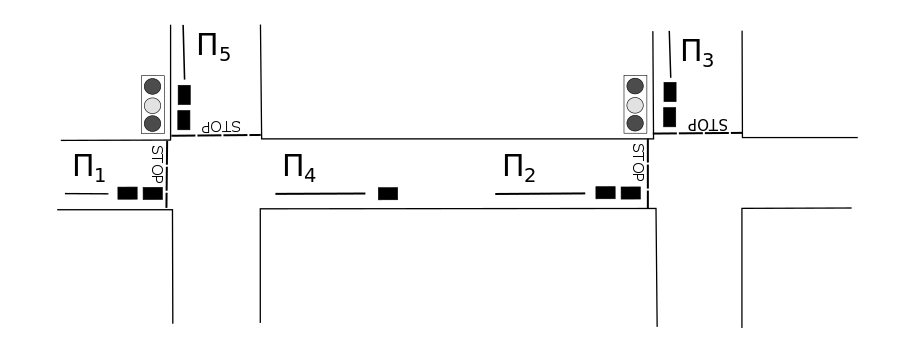
\includegraphics[scale=0.35]{Crossroads_grayscale.png}
\caption{Пример: тандем перекрестков}
\label{crossroads}
\end{figure}
Рассмотрим тандем из двух автомобильных перекрестков (рис.~\ref{crossroads}).
Машины, поступающие на первый перекресток в горизонтальном и вертикальном направлениях, образуют входящие потоки $\Pi_1$ и $\Pi_5$ соответственно. Каждая машина из потока $\Pi_1$, проезжая первый перекресток, немгновенно попадает на второй перекресток и образует поток машин $\Pi_2$. Также на второй перекресток поступают машины с вертикального направления и образуют входящий поток $\Pi_3$. Машины потока $\Pi_3$ имеют более низкий приоритет по сравнению с машинами горизонтального направления и могут проехать перекресток только если их количество превысит определенный числовой порог.

Для описания <<немгновенности>> перемещения машин между перекрестками удобно ввести промежуточный поток $\Pi_4$, состоящий из всех машин, обслуженных на первом перекрестке в горизонтальном направлении. 

Предполагается, что светофор на первом перекрестке имеет лишь два состояния $\{g_{1,1},g_{1,2}\}$: в состоянии $g_{1,1}$ машины потока $\Pi_1$ пропускаются фиксированное количество времени $\widetilde T^{(1,1)}$ (<<зеленый>> свет для $\Pi_1$); в состоянии $g_{1,2}$ --- простаивают в течение времени $\widetilde T^{(1,2)}$ (<<красный>> свет для $\Pi_1$). Светофор на втором перекрестке обслуживает по алгоритму с продлением: дополнительно к состоянию обслуживания потока $\Pi_3$ (состояние $g_{2,1}$), также имеется два состояния обслуживания потока $\Pi_2$ (состояния $\{g_{2,2},g_{2,3}\}$). Первое из них включается всегда после завершения обслуживания потока $\Pi_3$, а второе включается, если после очередного такта обслуживания потока $\Pi_2$ длина очереди $O_3$ не превосходит уровня $L$.
Длительности пребывания светофора на втором перекрестке в каждом из состояний суть $\widetilde T^{(2,1)}$, $\widetilde T^{(2,2)}$ и $\widetilde T^{(2,3)}$.

Для анализа тандема перекрестков удобно рассматривать его как единую систему массового обслуживания. Для этого предположим наблюдение за перекрестками только в (дискретные) моменты переключения состояния хотя бы одного из светофоров. Можно показать, что количество различных состояний у полученной системы конечно. Действительно, положим, например, за состояние объединенной системы вектор $(g^{(1)},g^{(2)}, s, t)$, где $g^{(1)}\in \{g_{1,1},g_{1,2}\}$~--- состояние $1$--го перекрестка, $g^{(2)}\in \{g_{2,1},g_{2,2},g_{2,3}\}$~--- состояние $2$--го перекрестка, $s \in \{0, 1, 2\}$~--- номер последнего сменившего состояние перекрестка (принимает значение $0$ в случае, если сменили состояние оба перекрестка) и $t \in \{0, 1, 2, \ldots, T\}$~--- количество времени, оставшееся у продолжающего обслуживание с прошлого такта перекрестка (принимает значение $0$, если принимает значение $0$ величина $s$). Здесь $T$~--- максимальная длительность нахождения каждого из светофоров в одном состоянии. Тогда количество различных состояний не трудно посчитать и оно не будет превышать величины  $2\times 3 \times 3 \times T$.

Отметим, что при прохождении перекрестков машины предполагаются движущимися только в прямом направлении, то есть перемешивания потоков не допускается. Таким образом, поток $\Pi_5$ не представляет интереса для дальнейшего исследования системы и может быть исключен из рассмотрения.
\begin{figure}[ht]
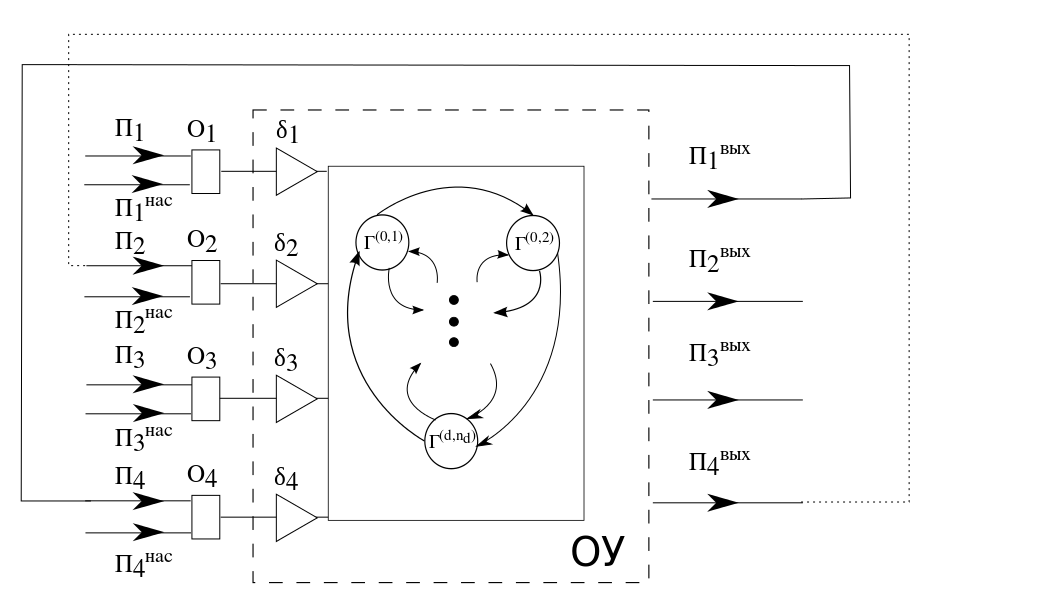
\includegraphics[scale=0.3]{SystemScheme.png} 
\caption{Структурная схема системы обслуживания}
\label{SystemScheme}
\end{figure}
В общем виде система массового обслуживания, описывающая тандем перекрестков, имеет следующий вид (рис.~\ref{SystemScheme}).
В систему с одним обслуживающим устройством поступают потоки $\Pi_1$, $\Pi_2$, $\Pi_3$  и $\Pi_4$. Требования по потоку $\Pi_j$ становятся в соответствующую очередь $O_j$ с неограниченной вместимостью, $j\in \{1, 2, 3, 4\}$. Для $j \in \{1, 2, 3\}$ дисциплина очереди $O_j$, поддерживаемая устройством $\delta_j$, имеет тип FIFO (First In First Out). Таким образом, для обслуживания из соответствующей очереди выбирается то требование, которое пришло раньше. Дисциплина очереди $O_4$ будет описана ниже. Входные потоки $\Pi_1$ и $\Pi_3$ формируются внешней средой, которая, будем предполагать, имеет только одно состояние, то есть вероятностная структура потоков не меняется с течением времени. Требования потоков $\Pi_1$ и $\Pi_3$ формируют независимые между собой неординарные пуассоновские потоки, то есть  стационарные, без последействия и ординарные потоки групп требований. Интенсивности соответствующих простейших потоков для $\Pi_1$ и $\Pi_3$ будем обозначать $\lambda_1$ и $\lambda_3$, а распределение числа заявок в группе по потоку $\Pi_j$ будем описывать производящей функцией
\begin{equation}
f_j(z) = \sum_{\nu=1}^{\infty} p_{\nu}^{(j)} z ^{\nu}, \quad j\in \{1,3\},
\label{GeneratingFunc}
\end{equation}
которая предполагается аналитической при любом $z\in \mathbb{C}$ таком, что $|z|<(1+\varepsilon)$, $\varepsilon>0$. Величина $p_{\nu}^{(j)}$ определяет вероятность того, что по потоку $\Pi_j$ число требований в группе равно $\nu$. Обслуженные требования потока $\Pi_1$ поступают на повторное обслуживание, формируя на выходе поток $\Pi_4$. Обслуженные требования потока $\Pi_4$ в свою очередь поступают на повторное обслуживание, формируя при этом поток $\Pi_2$. Потоки $\Pi_2$ и $\Pi_3$ являются конфликтными, что означает запрет на одновременное обслуживание требований этих потоков и, следовательно, исследование системы не может быть сведено к задаче с меньшим числом потоков. 

В каждый момент времени обслуживающее устройство находится в одном из конечного множества состояний $\Gamma=\{\Gamma^{(k,r)} \colon k=\overline{0,d}; r=\overline{1,n_k}\}$ с заданными натуральными числами $d$, $n_0$, $n_1$, $\ldots$, $n_d$. В каждом состоянии $\Gamma^{(k,r)}$ обслуживающее устройство находится в течение неслучайного времени $T^{(k,r)}$. 
Введем непересекающиеся подмножества $\Gamma^{\mathrm{I}}$, $\Gamma^{\mathrm{II}}$, $\Gamma^{\mathrm{III}}$ и $\Gamma^{\mathrm{IV}}$ множества $\Gamma$ следующим образом. 
В состоянии $\Gamma^{(k,r)} \in \Gamma^{\mathrm{\Rmnum{1}}}$ 
обслуживаются только требования из очередей $O_1$, $O_2$ и $O_4$.
В состоянии $\gamma \in \Gamma^{\mathrm{\Rmnum{2}}}$ обслуживаются только требования из очередей $O_2$ и $O_4$.
В состоянии $\gamma \in \Gamma^{\mathrm{\Rmnum{3}}}$ обслуживаются только требования из очередей $O_1$, $O_3$ и $O_4$.
В состоянии $\gamma \in \Gamma^{\mathrm{\Rmnum{4}}}$ обслуживаются только требования из очередей $O_3$ и $O_4$.
Тогда множество $\Gamma$ есть объединение $\Gamma = \Gamma^{\mathrm{I}} \cup \Gamma^{\mathrm{II}} \cup \Gamma^{\mathrm{III}} \cup \Gamma^{\mathrm{III}}$ непересекающихся подмножеств. Также в дальнейшем нам понадобятся множества ${}^1\Gamma=\Gamma^{\mathrm{\Rmnum{1}}} \cup \Gamma^{\mathrm{\Rmnum{3}}}$, 
${}^2\Gamma=\Gamma^{\mathrm{\Rmnum{1}}} \cup \Gamma^{\mathrm{\Rmnum{2}}}$,
${}^3\Gamma=\Gamma^{\mathrm{\Rmnum{3}}} \cup \Gamma^{\mathrm{\Rmnum{4}}}$. 

\begin{figure}[t]\centering
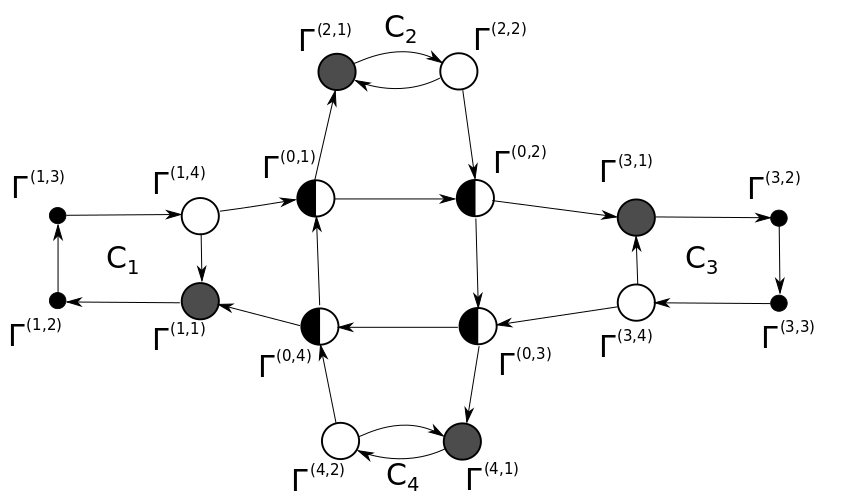
\includegraphics[scale=0.35]{GraphScheme3_grayscale.png} 
\caption{Класс графов переходов. Незакрашенные вершины являются выходными вершинами, большие черные вершины --- входные, небольшие черные --- нейтральные, наполовину закрашенным вершинам соответствуют состояния продления}
\label{GraphScheme}
\end{figure}

Смена состояний обслуживающего устройства осуществляется по следующему правилу. Множество состояний $C_k = \{\Gamma^{(k,r)} \colon r=\overline{1,n_k}\}$ будем называть $k$-м циклом, $k=\overline{1,d}$ (Рис. \ref{GraphScheme}). Состояние вида $\Gamma^{(0,r)}$ будем называть состоянием продления, $r=\overline{1,n_0}$. Положим $r \oplus_k 1 = r+1$ для $r=\overline{1,n_k-1}$ и $r \oplus_k 1 = 1$ при $r=n_k$, $k = \overline{0,d}$. В цикле $C_k$ выделим подмножества $C_k^{\mathrm{O}}$ выходных, $C_k^{\mathrm{I}}$ входных и $C_k^{\mathrm{N}} = C_k \setminus (C_k^{\mathrm{O}} \cup C_k^{\mathrm{I}})$ нейтральных состояний. Тогда после состояния $\Gamma^{(k,r)} \hm\in C_k\setminus C_k^{\mathrm{O}}$ обслуживающее устройство переходит в состояние $\Gamma^{(k,r \oplus_k 1)}$ того же цикла $C_k$. При $\Gamma^{(k,r)}$ принадлежащем множеству $C_k^{\mathrm{O}}$ прибор переходит в состояние $\Gamma^{(k,r \oplus_k 1)}$, если число требований в очереди $O_3$ в момент переключения больше заданного порога $L$. В противном случае, то есть если число требований в очереди $O_3$ меньше либо равно $L$, новое состояние прибора будет состоянием продления $\Gamma^{(0,r_1)}$, где $r_1=h_1(\Gamma^{(k,r)})$ и $h_1(\cdot)$~--- заданное отображение множества $\bigcup\limits_{k=1}^d C_k^{\mathrm{O}}$ во множество $\{1,2,\ldots, n_0\}$. После состояния $\Gamma^{(0,r)}$ выбирается состояние того же вида $\Gamma^{(0,r_2)}$, если число требований в очереди $O_3$ меньше или равно $L$, где $r_2=h_2(r)$ и $h_2(\cdot)$~--- заданное отображение множества $\{1,2, \ldots, n_0\}$ на себя; в противном случае включается входное состояние $\Gamma^{(k,r_3)} \in C_k^{\mathrm{I}}$, где $\Gamma^{(k,r_3)}=h_3(r)$ и $h_3(\cdot)$~--- заданное отображение множества $\{1,2, \ldots, n_0\}$ на множество  $\bigcup\limits_{k=1}^d C_k^{\mathrm{I}}$. Считается, что все состояния продления $\Gamma^{(0,r)}$ принадлежат множеству ${}^2 \Gamma$, а также верны соотношения $C_k^\mathrm{O}\subset {}^2 \Gamma$ и $C_k^\mathrm{I}\subset {}^3 \Gamma$. Также будем предполагать, что все циклы имеют ровно одно входное и одно выходное состояние. И последним предположением является то, что все вершины продления образуют один цикл, то есть можем положить $h_2(r)=r\oplus_0 1$.


%\subsection{Допустимые графы переходов состояний ОУ}

Таким образом, смена состояний обслуживающего устройства задается соотношением:
\begin{equation}
h(\Gamma^{(k,r)},y) = 
\begin{cases}
\Gamma^{(k,r \oplus_k 1)},&  \text{если } (\Gamma^{(k,r)}\in C_k\setminus C_k^{\mathrm{O}}) \\ 
&\text{ или } (\Gamma^{(k,r)}\in C_k^{\mathrm{O}} \text{ \& } y>L);\\
%\Gamma^{(k,r \oplus_k 1)},& \quad \text{ если } \Gamma^{(k,r)}\in C_k^{\mathrm{O}} \text{ и } y>L;\\
\Gamma^{(0,h_1(\Gamma^{(k,r)}))},&  \text{если } \Gamma^{(k,r)}\in C_k^{\mathrm{O}} \text{ и } y\leqslant L;\\
\Gamma^{(0,r \oplus_0 1)},&  \text{если } k=0 \text{ и } y\leqslant L;\\
h_3(r),&  \text{если } k=0 \text{ и } y > L.
\end{cases}
\label{hLaw}
\end{equation}















% \begin{figure}[t]
% 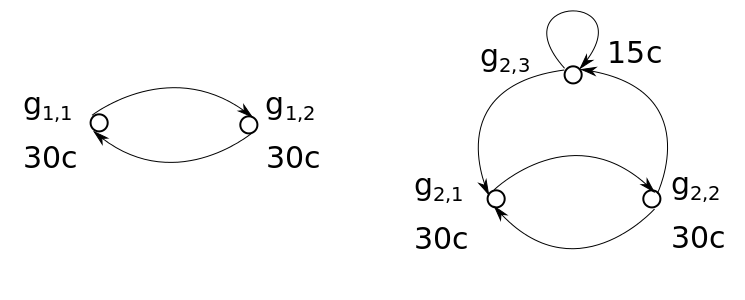
\includegraphics[scale=0.4]{SystemStates.png} 
% \caption{Числовой пример тандема перекрестков. Левый граф соответствует первому перекрестку, правый~--- второму}
% \label{SystemStates}
% \end{figure}


% Теперь продемонстрируем на конкретном числовом примере выделение циклов и состояний продления. Пусть изменение состояний перекрестков и время пребывания (в секундах для определнности) в каждом из состояний задается графами на рис. \ref{SystemStates}.

% За начальное состояние объединенной системы примем $\Gamma_0=(g_{1,1},g_{2,1},0,0)$, то есть первый перекресток находится в состоянии $g_{1,1}$, второй~--- в состоянии $g_{2,1}$, и оба только начали свою работу в своем состоянии (этот факт моделируется равенствами $s=0$ и $t=0$). Следующая смена состояний случится у обоих перекрестков одновременно и приведет к следующему состоянию $(g_{1,2},g_{2,2}, 0, 0)$. Далее смена состояний произойдет также у первого и второго перекрестков, однако второй перекресток может перейти как в состояние $g_{2,1}$, так и в состояние продления $g_{2,3}$. Таким образом следущим состоянием тандема будет либо опять $(g_{1,1},g_{2,1},0,0)$, либо $(g_{1,1},g_{2,3},0,0)$. Продолжая рассуждения аналогичным образом, получим следущий список всех возможных состояний системы:

% \begin{align}
% (g_{1,1},g_{2,1},0,0)&=\Gamma^{(1,1)} ,& \quad (g_{1,2},g_{2,2},0,0)&=\Gamma^{(1,2)} ,& \quad (g_{1,1},g_{2,3},0,0)&=\Gamma^{(0,1)}, \\
% (g_{1,1},g_{2,3},15,2)&=\Gamma^{(0,2)} ,& \quad (g_{1,2},g_{2,3},0,0)&=\Gamma^{(0,3)} ,& \quad (g_{1,2},g_{2,3},15,2)&=\Gamma^{(0,4)}, \\
% (g_{1,2},g_{2,1},15,2)&=\Gamma^{(4,1)} ,& \quad (g_{1,1},g_{2,1},15,1)&=\Gamma^{(4,2)} ,& \quad (g_{1,1},g_{2,2},15,2)&=\Gamma^{(4,3)}, \\
% (g_{1,2},g_{2,2},15,1)&=\Gamma^{(4,4)} ,& \quad (g_{1,2},g_{2,3},15,2)&=\Gamma^{(0,5)} ,& \quad (g_{1,2},g_{2,1},0,0)&=\Gamma^{(3,1)}, \\
% (g_{1,1},g_{2,2},0,0)&=\Gamma^{(3,2)} ,& \quad (g_{1,1},g_{2,1},15,2)&=\Gamma^{(2,1)} ,& \quad (g_{1,2},g_{2,1},15,1)&=\Gamma^{(2,2)}, \\
% (g_{1,2},g_{2,2},15,2)&=\Gamma^{(2,3)} ,& \quad (g_{1,1},g_{2,2},15,1)&=\Gamma^{(2,4)}. & &
% \end{align}

% В соответсвии с приведенными выше обозначениями, множества $C_1$, $C_2$, $C_3$, $C_4$, а также множество состояний продления строятся однозначным образом. 
% Множествами входных состояний будут 
% $C_1^{\mathrm{I}}=\{\Gamma^{(1,1)}\}$, 
% $C_2^{\mathrm{I}}=\{\Gamma^{(2,1)}\}$, $C_3^{\mathrm{I}}=\{\Gamma^{(3,1)}\}$ и $C_4^{\mathrm{I}}\hm=\{\Gamma^{(4,1)}\}$. Множествами выходных состояний будут 
% $C_1^{\mathrm{O}}=\{\Gamma^{(1,2)}\}$, $C_2^{\mathrm{O}}=\{\Gamma^{(2,4)}\}$, $C_3^{\mathrm{O}}=\{\Gamma^{(3,2)}\}$ и $C_4^{\mathrm{O}}=\{\Gamma^{(4,4)}\}$. 
% Функции $h_1(\cdot)$, $h_2(\cdot)$ и $h_3(\cdot)$ задаются поточечно:
% \begin{equation*}
% h_1(\Gamma^{(1,2)})=1, \quad h_1(\Gamma^{(2,4)})=2, \quad h_1(\Gamma^{(3,2)})=3, \quad h_1(\Gamma^{(4,4)})=5,
% \end{equation*}
% \begin{equation*}
% h_2(1)=2, \quad h_2(2)=3, \quad h_2(3)=4 \quad h_2(4)=1, \quad h_2(5)=1,
% \end{equation*}
% \begin{equation*}
% h_3(1)=\Gamma^{(2,1)}, \quad h_3(2)=\Gamma^{(3,1)}, \quad h_3(3)=\Gamma^{(4,1)} \quad h_3(4)=\Gamma^{(1,1)}, \quad h_3(5)=\Gamma^{(1,1)}.
% \end{equation*}
% Этим завершается построение числового примера.




























\section{Математическая модель}

Описанная выше система массового обслуживания должна рассматриваться как кибернетическая управляющая система обслуживания (см. \cite{Zorine:2011:2}). Схема управляющей системы приведена на рис. \ref{SystemScheme}. На схеме присутствуют следующие блоки: 1) внешняя среда с одним состоянием; 2) входные полюса первого типа~--- входные потоки $\Pi_1$, $\Pi_2$, $\Pi_3$, $\Pi_4$; 3) входные полюса второго типа~--- потоки насыщения $\Pi_1^{\mathrm{\text{нас}}}$, $\Pi_2^{\mathrm{\text{нас}}}$, $\Pi_3^{\mathrm{\text{нас}}}$, $\Pi_4^{\mathrm{\text{нас}}}$; 4) внешняя память~--- очереди $O_1$, $O_2$, $O_3$, $O_4$; 5) устройство по переработкe информации внешней памяти~--- устройства по поддержанию дисциплины очереди $\delta_1$, $\delta_2$, $\delta_3$, $\delta_4$; 6) внутренняя память~--- обслуживающее устройство (ОУ); 7) устройство по переработке информации во внутренней памяти~--- граф смены состояний; 8) выходные полюса $\Pi_1^{\mathrm{\text{вых}}}$, $\Pi_2^{\mathrm{\text{вых}}}$, $\Pi_3^{\mathrm{\text{вых}}}$, $\Pi_4^{\mathrm{\text{вых}}}$. Координатой блока является номер этого блока на схеме. 

Для задания информации блоков введем следующие величины и элементы, а также укажем множества их возможных значений. В качестве дискретной временной шкалы выберем последовательность $\tau_0=0$, $\tau_1$, $\tau_2$, $\ldots$ моментов смены состояния обслуживающего устройства. Обозначим $\Gamma_i$, $i\geqslant 1$, из множества $\Gamma$ состояние обслуживающего устройства в течение времени $\left(\tau_{i-1};\tau_i\right]$ и $\Gamma_0\in \Gamma$~--- в момент времени $\tau_0$, количество $\varkappa_{j,i} \in \mathbb{Z}_+ $, $i\geqslant 0$, требований в очереди $O_j$ в момент времени $\tau_i$, количество $\eta_{j,i} \in \mathbb{Z}_+$, $i\geqslant 0$, требований, поступивших в очередь $O_j$ по потоку $\Pi_j$ в течение времени $\left(\tau_{i};\tau_{i+1}\right]$, количество $\xi_{j,i} \in \mathbb{Z}_+$, $i\geqslant 0$, требований по потоку насыщения $\Pi^{\mathrm{\text{нас}}}_j$ в течение времени $\left(\tau_{i};\tau_{i+1}\right]$, количество $\overline{\xi}_{j,i}\in \mathbb{Z}_+$, $i\geqslant 0$, реально обслуженных требований по потоку $\Pi_j$ в течение времени $\left(\tau_{i};\tau_{i+1}\right]$; $j=\overline{1,4}$.

Закон изменения состояния обслуживающего устройства будем предполагать заданным соотношением 
\begin{equation*}
\Gamma_{i+1}=h(\Gamma_i,\varkappa_{3,i}),
%\label{gammaFunc}
\end{equation*}
где отображение $h(\cdot,\cdot)$ определено в \eqref{hLaw}.
Для определения длительности $T_{i+1}$ состояния обслуживающего устройства в течение времени $\left(\tau_{i};\tau_{i+1}\right]$ удобно ввести функцию $h_T(\cdot,\cdot)$:
\begin{equation*}
T_{i+1}=h_T(\Gamma_i,\varkappa_{3,i})= T^{(k,r)},\quad  \text{ где $k$ и $r$ таковы, что } \Gamma^{(k,r)}=\Gamma_{i+1}.
%\label{timeLaw}
\end{equation*}
Функциональная зависимость
\begin{equation}
\overline{\xi}_{j,i}=\min\{\varkappa_{j,i}+\eta_{j,i},\xi_{j,i}\}, \quad j\in \{1,2,3\},
\label{saturationEq}
\end{equation}
между величиной $\overline{\xi}_{j,i}$ и величинами $\varkappa_{j,i}$, $\eta_{j,i}$, $\xi_{j,i}$ реализует стратегию механизма обслуживания требований. Далее, поскольку 
\begin{equation*}
\varkappa_{j,i+1}=\varkappa_{j,i}+\eta_{j,i}-\overline{\xi}_{j,i}, \quad  j\in \{1,2,3\},
\end{equation*}
то из выражения \eqref{saturationEq} следует соотношение
\begin{equation*}
\varkappa_{j,i+1}=\max\{{0,\varkappa_{j,i}+\eta_{j,i}-\xi_{j,i}}\}, \quad j\in \{1,2,3\}.
%\label{queuesFunc}
\end{equation*}
Из формулировки поставленной задачи (см. также структурную схему на рис.~\ref{SystemScheme}) следуют соотношения для потока $\Pi_4$:
\begin{equation*}
\eta_{4,i} = \min\{\xi_{1,i}, \varkappa_{1,i}+\eta_{1,i}\}, \quad \varkappa_{4,i+1}=\varkappa_{4,i}+\eta_{4,i}-\eta_{2,i}, \quad \xi_{4,i} = \varkappa_{4,i}.
%\label{FourthFunc}
\end{equation*}

Нелокальное описание входных потоков и потоков насыщения состоит в указании некоторых свойств условных распределений выделенных дискретных компонент $\eta_i=(\eta_{1,i},\eta_{2,i}, \eta_{3,i}, \eta_{4,i})$ и $\xi_i=(\xi_{1,i}, \xi_{2,i}, \xi_{3,i}, \xi_{4,i})$ маркированных точечных процессов \linebreak $\{(\tau_i, \nu_i, \eta_i); i\geqslant 0\}$ и $\{(\tau_i, \nu_i, \xi_i); i\geqslant 0\}$ при фиксированных значениях метки $\nu_i = (\Gamma_i;\varkappa_i)$, где $\varkappa_i=(\varkappa_{1,i},\varkappa_{2,i},\varkappa_{3,i},\varkappa_{4,i})$. 
Введем функции $\varphi_1(\cdot,\cdot)$ и $\varphi_3(\cdot,\cdot)$ из разложений 
\begin{equation*}
\sum_{\nu=0}^{\infty} z^\nu\varphi_j(\nu,t) = \exp\{\lambda_j t (f_j(z)-1)\},
\end{equation*}
где $f_j(z)$ определены выражением \eqref{GeneratingFunc}, $j \in \{1,3\}$. Функция $\varphi_j(\nu,t)$ по своему смыслу есть вероятность поступления $\nu=0$, $1$, $\ldots$ требований по потоку $\Pi_j$ за время $t \geqslant 0$. Положим $\varphi_j(\nu,t)$ равной нулю при $\nu < 0$. Функцию $\psi(\cdot,\cdot,\cdot)$ зададим формулой
\begin{equation*}
\psi(k;y,u)=C_y^k u^k (1-u)^{y-k}.	
\end{equation*}
По своему смыслу $\psi(k;y,u)$ есть вероятность поступления $k$ требований по потоку $\Pi_2$ при условии, что очередь $O_4$ содержит $y$ требований и обслуживающее устройство находится в состоянии $\Gamma^{(k,r)}$, так что $u=p_{k,r}$. При нарушении условия $ 0\leqslant k \leqslant y$ положим $\psi(k;y,u)$ равной нулю.

Пусть $a=(a_1, a_2, a_3, a_4) \in \mathbb{Z}_+^4$ и $x=(x_1, x_2, x_3, x_4) \in \mathbb{Z}_+^4$. Тогда из постановки задачи на содержательном уровне следует, что при фиксированном значении метки $\nu_i=(\Gamma^{(k,r)}; x)$ вероятность $\varphi(a,k,r,x)$ одновременного выполнения равенств $\eta_{1,i}=a_1$, $\eta_{2,i}=a_2$, $\eta_{3,i}=a_3$, $\eta_{4,i}=a_4$ есть 
\begin{multline*}
\varphi_1(a_1,h_T(\Gamma^{(k,r)},x_3)) \times \psi(a_2,x_4, p_{\tilde{k},\tilde{r}}) \times \\ \times \varphi_3(a_3,h_T(\Gamma^{(k,r)},x_3))
\times \delta_{a_4,\min{\{\ell(\tilde{k},\tilde{r},1), x_1+a_1}\}},
%\label{conditionProbOne}
\end{multline*}
где $\tilde{k}$ и $\tilde{r}$ таковы, что $\Gamma^{(\tilde{k},\tilde{r})}=h(\Gamma^{(k,r)},x_3)$ и $\delta_{i,j}$ есть символ Кронекера:
%\begin{equation*}
$$
\delta_{i,j}=
\begin{cases} 
1,& \quad \text{ если $i=j$,}\\
0,& \quad \text{ если $i\neq j$.}
\end{cases}
$$%\end{equation*}
Пусть $b=(b_1, b_2, b_3, b_4) \in \mathbb{Z}_+^4$. Из содержательной постановки задачи также следует, что вероятность $\zeta(b, k, r, x)$ одновременного выполнения равенств $\xi_{1,i}=b_1$, $\xi_{2,i}=b_2$, $\xi_{3,i}=b_3$, $\xi_{4,i}=b_4$ при фиксированном значении $(\Gamma^{(k,r)}; x)$ метки $\nu_i$ есть
\begin{equation}
\delta_{b_1,\ell(\tilde{k},\tilde{r},1)} \times \delta_{b_2,\ell(\tilde{k},\tilde{r},2)} \times 
\delta_{b_3,\ell(\tilde{k},\tilde{r},3)} \times \delta_{b_4,x_4}.
\label{conditionProbTwo}
\end{equation}
Из формулы \eqref{conditionProbTwo} следует для $j\in \{1, 2, 3\}$, что вероятность события $\xi_{j,i}=0$ равна $1$ в случае $h(\Gamma^{(k,r)},x_3)\notin {}^j\Gamma$ и что вероятность события $\xi_{j,i}=\ell(\tilde{k},\tilde{r},j)$ равна $1$, если $\Gamma^{(\tilde{k},\tilde{r})}=h(\Gamma^{(k,r)},x_3)\in {}^j\Gamma$.






В предыдущих работах была исследована последовательность $\{(\Gamma_i, \varkappa_{1,i},\varkappa_{3,i}); i \geqslant 0\}$ и была доказана ее марковость. Также для нее найдено достаточное условие существования стационарного распределения в виде выполнения системы неравенств:
\begin{equation}
\min_{k=\overline{0,d}} { \frac{\sum_{r = 1}^{n_k} \ell(k,r,1) }{\lambda_1 f_1'(1) \sum_{r=1}^{n_k} T^{(k,r)} }}>1, \quad 
\min_{k=\overline{1,d}} { \frac{\sum_{r = 1}^{n_k} \ell(k,r,3) }{\lambda_3 f_3'(1) \sum_{r=1}^{n_k} T^{(k,r)} }}>1.
\label{sufficient:double}
\end{equation}









\section{Исследование системы управления тандемом с помощью имитационной модели}

\subsection{ОПИСАНИЕ ИМИТАЦИОННОЙ МОДЕЛИ}
На основании результатов анализа математической модели системы была построена компьютерная имитационная модель для тандема перекрестков. Первоначально фиксируются параметры входных потоков:
$\lambda_j$,  $p_{\nu}^{(j)}>0$ ($j=1,3$, $\nu=1$, $2$, $\ldots$); параметры перекрестков: $\mu_1$, $\mu_2$,  $\mu_3$, $\mu_4$, $\mu_{prolong}$; параметры алгоритма управления перекрестками: $\widetilde T^{(1,1)}$, $\widetilde T^{(1,2)}$, $\widetilde T^{(2,1)}$, $\widetilde T^{(2,2)}$, $\widetilde T^{(2,3)}$, $L$. Здесь величины $\mu_1$, $\mu_2$ и $\mu_3$  описывают интенсивности обслуживания требований потоков $\Pi_1$, $\Pi_2$ и $\Pi_3$ соответственно, а $\mu_{prolong}$ --- интенсивность обуслуживания требований потока $\Pi_2$ при продлении. Величина $\mu_4$ определяет вероятность $p_{k,r}$ для состояния $\Gamma^{(k,r)}$ продолжительностью $T^{(k,r)}$ по формуле $p_{k,r} = 1- \exp{(- T^{(k,r)} \mu_4)}$.  

Следующим шагом работы программы является объединение множеств состояний двух перекрестков и создание общего множества состояний для единой системы массового обслуживания. Это объединение осуществляется по схеме, описанной в постановке задачи. Также результатом работы на данном этапе является граф переходов из одного состояния обслуживающего устройства в другое.

Для решения вопроса о моменте завершения переходных процессов в системе производилась одновременная имитация системы с двумя различными начальными условиями. Во-первых, производится имитация системы при отсутствии ожидающих или находящихся на обслуживании требований в системе в момент начала ее функционирования, а во-вторых -- при наличии некоторого случайного количества требований, находящихся в каждой очереди  в момент начала функционирования системы. Систему при таких ненулевых начальных очередях будем в дальнейшем называть смещенной и величины, подсчитанные для нее, будем обозначать верхним индексом <<+>>. Напротив, систему при пустых начальных очередях называем несмещенной и относящиеся к ней величины выделяем верхним индексом <<0>>. Ниже приведем алгоритм определения момента достижения системой стационарного режима по условию близости некоторых величин для смещенной и несмещенной систем. После завершения переходных процессов имитация продолжается лишь для несмещенной системы. В связи с этим, отсутствие у некоторой величины верхнего индекса <<0>> и <<+>> будет указывать на то, что ее значение подсчитывается для системы, находящейся в стационарном режиме. В случае отсутствия у величины индекса <<0>> или <<+>>, будем считать ее посчитанной для стационарного режима для несмещенной системы.

При построении компьютерной имитационной модели представленной системы в значительной степени применялся метод дискретных событий \cite{averill}. Так, в качестве состояния системы выбирается массив длин очередей (количеств требований в очередях) для смещенной и несмещенной систем, а также состояния, в которых находятся обслуживающие устройства. Событиями, которые могут происходить в системе и нуждаться в обработке, являются смены состояний обслуживающих устройств. 
Требования, поступающие на обслуживание по потокам $\Pi_1$ и $\Pi_3$, генерируются в начале каждого цикла моделирования в соответствии с законом их распределения. Для каждого требования запоминается момент его поступления в систему и ухода из нее, а также время до начала его обслуживания.


Пусть индекс $j\in \{1, 3\}$  указывает на номер потока, $n=1$, $2$, $\ldots$ указывает на номер такта функционирования системы.
 В имитационной модели отслеживаются значения следующих величин: $\gamma_{j,\nu}^0$ и $\gamma_{j,\nu}^+$ --- времена ожидания начала обслуживания требования с номером $\nu$ потока $\Pi_j$ в несмещенной и смещенной системах соответственно; $t_n$ --- длительность $n$-го такта;
 $\alpha^{0}_{\text{in}, j,n}$ и $\alpha^{+}_{\text{in},j,n}$  --- количество требований потока $\Pi_j$, пришедших за $n$-ый такт работы системы; 
 $\alpha^{+}_{\text{out},j,n}$ и $\alpha^{+}_{\text{out},j,n}$ --- количество требований потока $\Pi_j$, обслуженных на цикле с номером $n$ работы системы;  $\beta_{j,n}$ равно количеству требований, находящихся в очереди $O_j$, если обслуживающее устройство только начало обслуживать очередь $O_j$ и равно $0$ в остальных случаях; $\zeta_{j,\nu}$ --- время нахождения в системе требования $\nu$ потока $\Pi_j$ с момента его поступления и до момента выхода из системы. Заметим, что время $\zeta_{1,\nu}$ считается с момента поступления требования в систему в качестве требования потока $\Pi_1$ до момента выхода этого требования из системы после его обслуживания как требования потока $\Pi_4$.
 %Выделена переменная $t$, фиксирующая текущее время имитации. 
 Каждый раз, когда в системе происходит событие, оно обрабатывается и значения отслеживаемых величин изменяются. Имитация заканчивается, 
 если в системе не обнаружен стационарный режим за некоторое максимальное число тактов функционирования (рекомендуемое значение $100000$), или если количество тактов после достижения стационарного режима превышает некоторое фиксированное количество (рекомендуемое значение $100000$).
 

\subsection{АЛГОРИТМ ОПРЕДЕЛЕНИЯ МОМЕНТА ДОСТИЖЕНИЯ СТАЦИОНАРНОГО РЕЖИМА}
Как правило, под стационарным режимом на содержательном уровне понимают такой режим функционирования системы, устанавливающийся с течением времени, при котором выделенные ее характеристики остаются неизменными. Идея алгоритма определения момента достижения системой такого режима в данной работе заключается в следующем. Наблюдаем одновременно за динамикой смещенной и несмещенной систем и считаем для каждой из них некоторые усредненные величины. Момент, когда эти величины станут достаточно близки, считаем моментом окончания переходных процессов. Формализуем алгоритм. Зафиксируем параметры метода:  $1 < \delta_1$, $1 < \delta_2$ и $1 < \delta_3$. В конце каждого такта будем считать значения 
\begin{equation}
   \gamma_{j,\cdot}^0 = \frac{1}{\tilde{\mathcal{V}}_j^0}\sum_{\nu} \gamma_{j,\nu}^0, \quad \gamma_{j,\cdot}^+ = \frac{1}{\tilde{\mathcal{V}}_j^+}\sum_{\nu} \gamma_{j,\nu}^+ 
\end{equation}
средних времен ожидания обслуживания требований потоков $\Pi_j$ в несмещенной и смещенной системах соответственно. Кроме того, для несмещенной системы будем считать входящий и выходящий потоки:
\begin{equation}
    F^{0}_{\text{in},1} = \sum_n \alpha^{0}_{\text{in},1,n}, \quad 
    F^{0}_{\text{out},4} = \sum_n \alpha^{0}_{\text{out},4,n}
\end{equation}
\begin{equation}
    F^{0}_{\text{in},3} = \sum_n \alpha^{0}_{\text{in},3,n}, \quad 
    F^{0}_{\text{out},3} = \sum_n \alpha^{0}_{\text{out},3,n}.
\end{equation}


Стационарный режим считается достигнутым если выполнены все неравенства:
\begin{equation}
    \frac{|\gamma_{j,\cdot}^0 - \gamma_{j,\cdot}^+|}{\gamma_{j,\cdot}^0} < \delta_1, \quad
    \frac{F^{0}_{\text{in},1}}{F^{0}_{\text{out},4}} < \delta_2, \quad 
    \frac{F^{0}_{\text{in},3}}{F^{0}_{\text{out},3}} < \delta_3.
\end{equation}



\subsection{ПОКАЗАТЕЛИ КАЧЕСТВА РАБОТЫ СИСТЕМЫ}
После того, как стационарный режим в системе достигнут, можно приступать к оценке основных показателей качества функционирования системы. С этой целью продолжается процесс имитации, но только для несмещенной системы. Необходимо получить оценки для математического ожидания времени пребывания произвольного требования потока $\Pi_j$, $j\in \{1, 3\}$
%и математического ожидания количества требований в очереди $O_j$ в момент перехода обслуживающего устройства в состояние $^j\Gamma$ на произвольном цикле стационарного режима работы системы. 
За основу можно взять известные в теории вероятностей и математической статистике оценки соответствующих количественных характеристик. Оценки для времени пребывания в системе можно было бы построить по наблюдениям за каждым обслуженным требованием выделенной реализации потока $\Pi_j$.
%, а оценки для количества требований в очереди при переходе к состоянию обслуживания -- по наблюдениям за этой величиной на каждом цикле одной реализации. 
Итак, для каждого $j=1,3$  предлагаются следующие оценки для показателей качества работы системы по потоку $\Pi_j$ :
\begin{itemize}
    \item $\hat{E}\gamma_{j}=\frac{1}{\tilde{\mathcal{V}}_j}\sum_{\nu}\zeta_{j,\nu}$  -- оценка математического ожидания времени пребывания в системе произвольного требования потока $\Pi_j$.
\end{itemize}
Кроме того, имеет смысл получить оценки, характеризующие работу системы не по отдельному потоку, а для системы в целом. Для этого предлагается строить средние взвешенные оценки, где в качестве веса отдельному потоку  приписывается интенсивность поступления его требований, т.е. величина, равная $\lambda_j \sum_{\nu\geqslant1}\nu p_{\nu}^{(j)}$. Итак, имеем результирующую оценку целевой функции
\begin{itemize}
    \item $\hat{E}\gamma=\frac{\sum_{j\in\{1,3\}} (\lambda_j \sum_{\nu\geqslant1}\nu p_{\nu}^{(j)})\hat{E}\gamma_{j} }{\sum_{j\in\{1,3\}} \lambda_j \sum_{\nu\geqslant1}\nu p_{\nu}^{(j)}}$.
\end{itemize}



\subsection{АНАЛИЗ ОБЛАСТИ СТАЦИОНАРНОСТИ СИСТЕМЫ}
Для анализа функционирования тандема перекрестков были зафиксированы следующие параметры:
\begin{itemize}
    \item $\lambda_1=0.35$, $p_{1}^{(1)}=0.4$, $p_{2}^{(1)}=0.4$, $p_{3}^{(1)}=0.2$, $p_{\nu}^{(1)}=0$, $\nu > 3$;
    \item $(\widetilde{T}^{(1,1)}, \widetilde{T}^{(1,2)})=(20,10)$, $\mu_1 = 1.2$;
    \item $\boldsymbol{ \lambda_3=\{0.1, 0.2\}}$, $p_{1}^{(3)}=0.4$, $p_{2}^{(3)}=0.3$, $p_{3}^{(1)}=0.3$, $p_{\nu}^{(3)}=0$, $\nu > 3$;
        \item $\mu_4= 0.001$.
\end{itemize}
Здесь представлены два набора параметров, отличающихся лишь интенсивностью $\boldsymbol{\lambda_3}$ поступления групп требований по потоку $\Pi_3$. Для алгоритма управления перекрестками зафиксируем длительность $\widetilde{T}^{(2,3)}=10$ продления зеленого сигнала светофора для потока $\Pi_2$ и порог $L=10$ продления.

При фиксированном наборе параметров ($\lambda_3 = 0.1$ либо $\lambda_3=0.2$) проводилась серия экспериментов, в которых перебирались значения для длительности обслуживания  $\widetilde{T}^{(2,1)} = \{1, 5, 9, \ldots, 97\}$ требований потока $\Pi_3$ и длительности обслуживания $\widetilde{T}^{(2,2)} = \{1, 5, 9, \ldots, 97\}$ потока $\Pi_2$.

%0_1_thres_10_target
\begin{figure}[ht]
\centering
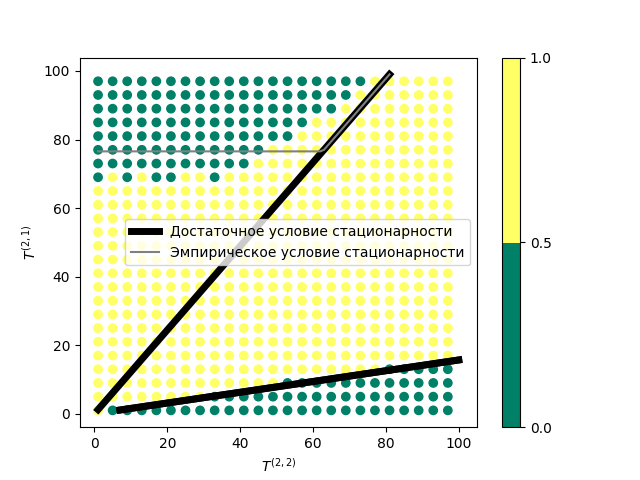
\includegraphics[scale=0.7]{0_1_thres_10_target_fact_.png} 
\caption{Область стационарности системы. $\lambda_3=0.1$, $L=10$}
\label{Experiment:stationar}
\end{figure}

\begin{figure}[ht]
\centering
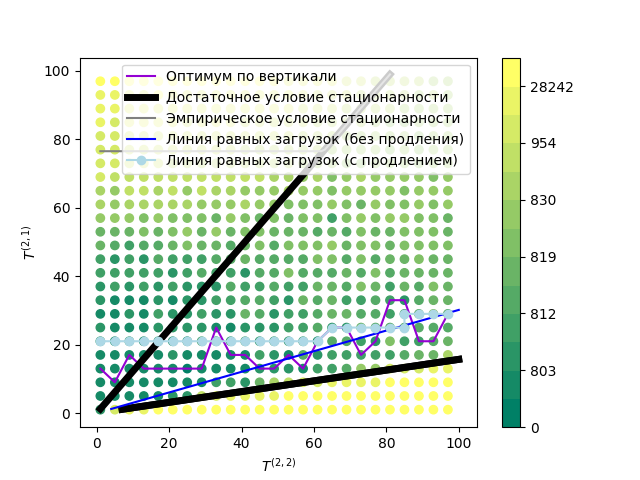
\includegraphics[scale=0.7]{0_1_thres_10_target.png} 
\caption{Графики равных квазизагрузок}
\label{Experiment:targets}
\end{figure}


\begin{figure}[ht]
    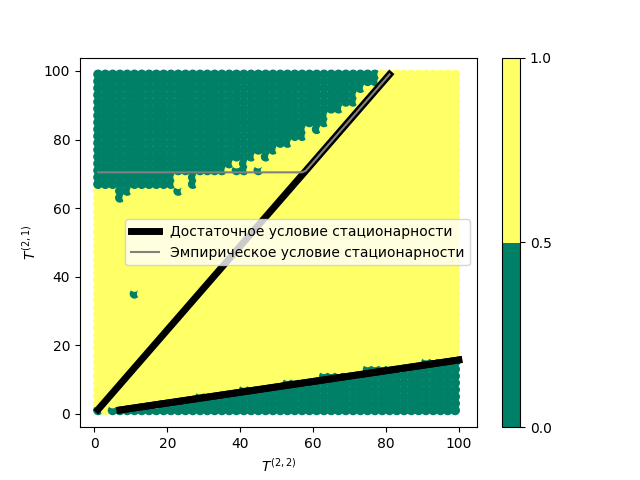
\includegraphics[scale=0.7]{0_1_thres_10_fact.png} 
\caption{Область стационарности для  $\lambda_1 = 0.1$}
\label{Experiment:intensities:one}
\end{figure}

\begin{figure}[ht]
    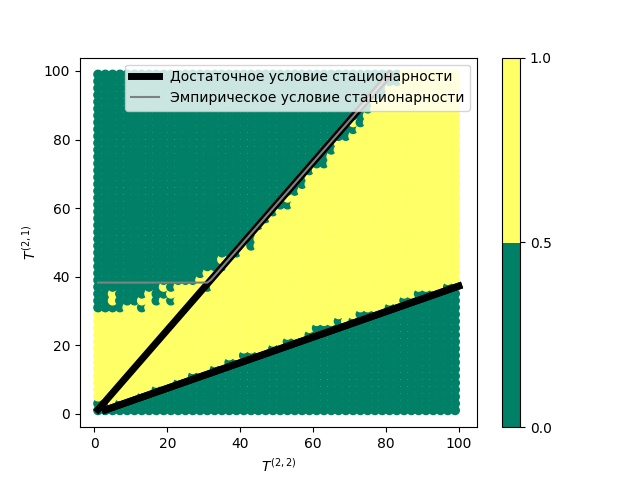
\includegraphics[scale=0.7]{0_2_thres_10_fact.png} 
\caption{Область стационарности для $\lambda_1 = 0.2$ (справа)}
\label{Experiment:intensities:two}
\end{figure}
% \begin{figure}[h]
% \begin{multicols}{2}
%     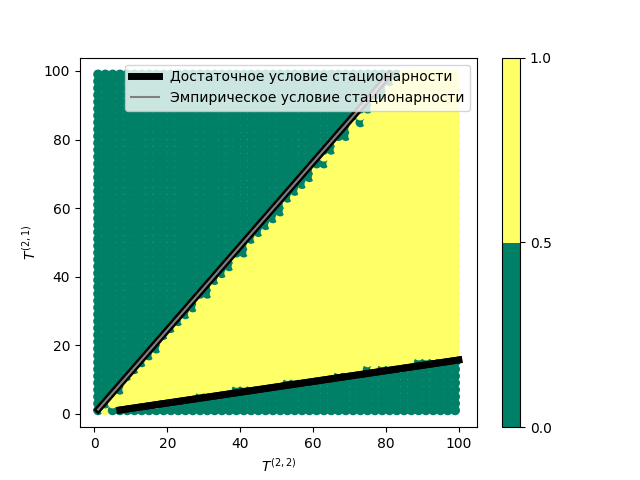
\includegraphics[width=1.15\linewidth]{0_1_thres_-1_fact.png}\par 
%     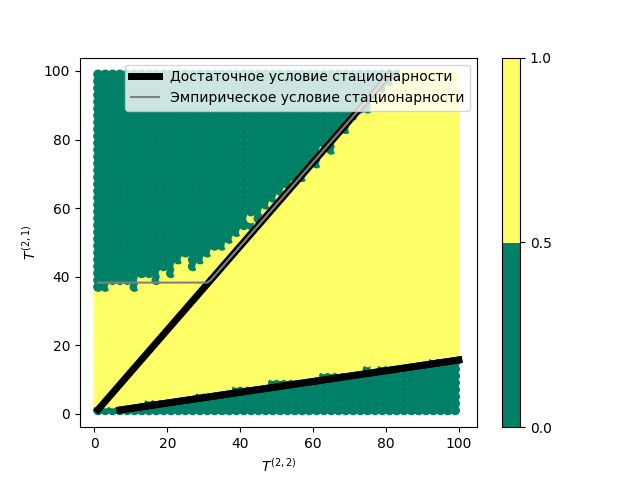
\includegraphics[width=1.15\linewidth]{0_1_thres_5_fact.png}\par 
%     \end{multicols}
% \caption{Области стационарности для порогов $L-1$ (слева) и $L=5$ (справа)}
% \end{figure}

% \begin{figure}[h]
% \begin{multicols}{2}
%     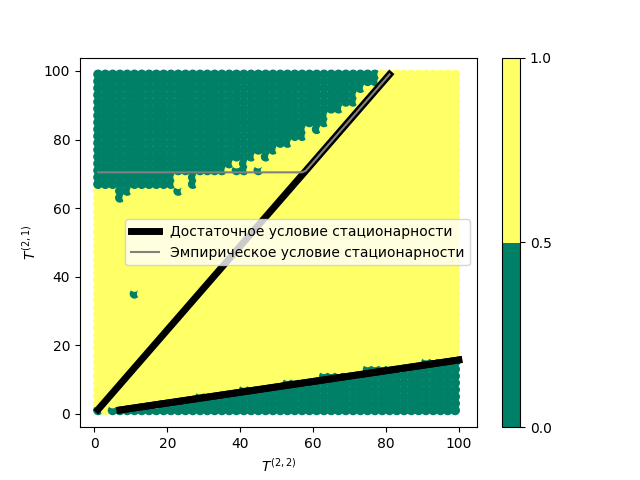
\includegraphics[width=1.15\linewidth]{0_1_thres_10_fact.png}\par
%     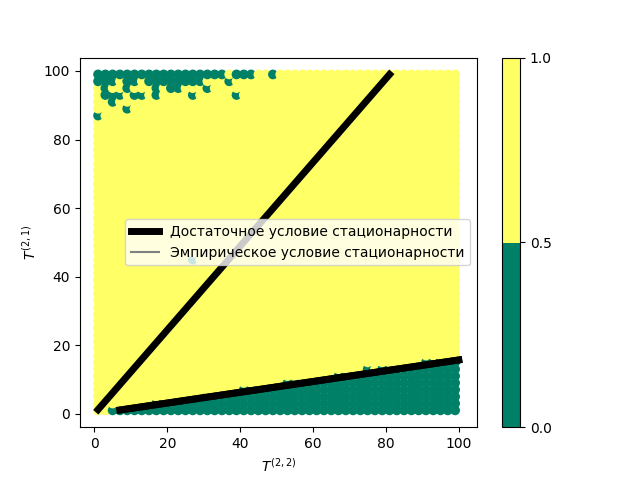
\includegraphics[width=1.15\linewidth]{0_1_thres_15_fact.png}\par
% \end{multicols}
% \caption{Области стационарности для порогов $L=10$, $L=15$}
% \end{figure}

На рис.~\ref{Experiment:stationar} представлены результаты экспериментов. По осям координат отложены значения $T^{(2,1)}$ длительности обслуживания требований потока $\Pi_3$ и значения $T^{(2,2)}$ длительности обслуживания требований потока $\Pi_2$. Желтым цветом обозначены точки, в которых было определено достижение системой стационарного режима. Темно-зеленым цветом обозначены случаи отсутствия стационарности. Кроме того на графике черным цветом изображена область стационарности, полученная из достаточных условий ~\ref{sufficient:double}. 

Из графика видно, что желтая область выходит далеко за границы черных линий. Это свидетельствует о том, что достаточное условие, полученное в работе аналитически, не является необходимым. Ввод дополнительного режима продления по высоко приоритетному потоку при отсутвии большого числа требований по низкоприоритетному потоку позволяет существенно расширить область стационарности системы. Интуитивно данный результат ожидаем: при отсутствии требований по одному из потоков, другой поток получает дополнительный временной <<запас>> для обслуживания за счет продления.

Также на графике изображена область, ограниченная снизу серой линией. Эта область получена эмпирическими рассуждениями и дает <<примерную>> оценку области стационарности для системы с продлением. Рассуждения для вывода этой границы основаны на подсчете <<среднего>> количества времени, освобождающегося для обслуживания требований потока $\Pi_2$ за счет продления.



Более детально результаты эксперимента представлены на рис.~\ref{Experiment:targets}. На этом рисунке каждому эксперименту соответствует посчитанная оценка средневзвешенной длительности ожидания одного требования. Чем более темным является цвет точки~--- тем лучше. Кроме присутствовавших на предыдущем рисунке границ, здесь присутствуют линии равных загрузок для случая циклического управления (синий цвет) и для случая циклического управления с продлением (голубой цвет). В работах \cite{Fedotkin:A:2009} и \cite{Fedotkin:Rachinskaya:2016} было отмечено, что оптимальные значение параметров с точки зрения средневзвешенного времени пребывания находится вблизи ломаной равных квазизагрузок. При условии отсутствия продления ($T^{(2,3)}=0$),  под загрузкой системы, например, по потоку $\Pi_1$ естественно понимать величину
\begin{equation}
\frac{(T^{(2,1)} + T^{(2,2)})\lambda_1 \sum_{\nu\geqslant 1}\nu p_{\nu}^{(1)}}{[\mu_2 T^{(2,2)}]}.
\end{equation}
Тогда ломаную равных квазизагрузок определим из условия равенства загрузки системы по потокам $\Pi_1$ и $\Pi_3$:
\begin{equation}
\frac{(T^{(2,1)} + T^{(2,2)})\lambda_1 \sum_{\nu\geqslant 1}\nu p_{\nu}^{(1)}}{[\mu_2 T^{(2,2)}]}=
    \frac{(T^{(2,1)} + T^{(2,2)})\lambda_3 \sum_{\nu\geqslant 1}\nu p_{\nu}^{(3)}}{[\mu_3 T^{(2,1)}]}
\end{equation}
График этой кривой изображен на рисунке~\ref{Experiment:targets} синим цветом. 


Далее встает вопрос о том, что считать загрузкой системы в случае присутствия продления по низкоприоритетному потоку $\Pi_3$. В данной работе под загрузкой будем понимать отношение общего числа пришедших требований по потоку ($\Pi_1$ или $\Pi_3$) к общему числу обслуженных требований по этому потоку. Аналитически посчитать эти величины сложно, поэтому на графике представлена кривая равных загрузок, посчитанная на основе экспериментальных данных. Как видно из рисунка, такая кривая лучше <<следует>> за оптимальными значениями параметров, нежели кривая равных квазизагрузок для циклического алгоритма.

Поясним, что значит кривая равных квазизагрузоу лучше <<следует>> за оптимальными значениями параметров. Поставим задачу: при фикисированном значении времени обслуживания потока $\Pi_2$ (величина $T^{(2,2)}$ на рис.~\ref{Experiment:targets}) найти такое значение времени обслуживания потока $\Pi_3$ (величина $T^{(2,1)}$ на рис.~\ref{Experiment:targets}), при котором достигается минимум средневзвешенного времени пребывания требования в системе. Фиолетовая линия на рис.~\ref{Experiment:targets} демонстрирует динамику этих значений при изменении времен $T^{(2,2)}$. Видно, что <<в среднем>> голубая линии лучше аппроксимирует фиолетовую кривую, чем синяя. Особенно в окрестности прямой $T^{(2,2)}=0$. 

Завершая анализ экспериментальных данных, отметим следующие наблюдения.
\begin{itemize}
    \item При увеличении интенсивности потока $\Pi_2$ (или, что то же самое, интенсивности потока $\Pi_1$), область  стационарности сужается (см.~Рис.~\ref{Experiment:intensities:one}, \ref{Experiment:intensities:two}).
    \item С увеличением порога $L$ продления, область стационарности увеличивается.
    %(см.~Рис.~). 
\end{itemize}

\section{Заключение}
В работе представлена математическая и имитационные модели для тандема систем обслуживания. При помощи кибернетического подхода сложная реальная система поддается строгому аналитическому исследованию. В то же время при помощи имитационной модели удалось подтвердить достаточные условия стационарности системы, полученные теоретически. Далее, удалось расширить известную область стационарности путем проведения численных экспериментов с использованием алгоритма определения момента наступления стационарного режима в имитационной модели. Анализ кривых равных загрузок для циклического и нециклического (с продлением) случаев показал, что область оптимальных параметров лежит между этими кривыми. Однако найти точное взаимное расположение кривых равных квазизагрузок и глобального оптимального набора параметров не удалось.

% Авторы - по алфавиту, сначала русскоязычные, затем остальные.
\begin{thebibliography}{100}
\bibitem{Klimenok:Dudin:2004} Бройер~Л., Дудин~А.Н., Клименок~В.И., Царенков~Г.В. Двухфазная система $BMAP|G|1|N \to PH|1|M-1-1$ с блокировкой // Автомат. и телемех.~--- 2004~--- \No{}~1.~--- С.~117–-130.
\bibitem{Zorine:2011:1} Зорин~А.В. Кибернетический подход к построению и анализу математической модели тандема двух перекрестков // Проблемы теоретической кибернетики. Материалы XVI Международной конференции (Нижний Новгород, 20-25 июня 2011 г.), Нижний Новгород: Изд-во Нижегородского университета.~--- 2011.~--- С.~179--183.
\bibitem{Zorine:2011:2} Зорин~А.В. Устойчивость тандема систем обслуживания с бернуллиевским немгновенным перемещением требований // Теория вероятностей и математическая статистика, вып. 84.~--- 2011.~--- С.~163--176.
\bibitem{Klimenok:2015} Клименок~В.И., Савко~Р.Ч. Двухфазная система с повторными попытками и нетерпеливостью запросов // Автомат. и телемех. 2015.~--- \No{}~8.~--- С.~78-–93. 
\bibitem{Klimenok:2010} Клименок~В.И., Тарамин~О.С. Двухфазная система обслуживания с групповым марковским потоком и повторными вызовами // Автомат. и телемех.~--- 2010.~--- \No~1.~--- С.~3–-17 
\bibitem{Klimenok:2011} Клименок~В.И., Тарамин~О.С. Двухфазная система $GI/PH/1 \to /PH/1/0GI/PH/1 \to /PH/1/0$ с потерями // Автомат. и телемех.~--- 2011.~--- \No{}~5.~--- C.~113-–126.
\bibitem{Kocheganov:2017:3} Кочеганов~В.М., Зорин~А.В. Анализ потоков первичных требований в тандеме при циклическом управлении с продлением // Информационные технологии и математическое моделирование (ИТММ--2017): Материалы XVI Международной конференции имени А.Ф. Терпугова (29 сентября -- 3 октября 2017 г.) -- Томск: Изд-во~НТЛ.~--- 2017.~--- Ч.~1.~--- С.81--87.
\bibitem{Kocheganov:2015:1} Кочеганов~В.М., Зорин~А.В. Вероятностная модель тандема систем массового обслуживания с циклическим управлением с продлением // Теория вероятностей, случайные процессы, математическая статистика и приложения: материалы Междунар. науч. конф., посвящ. 80-летию проф., д-ра физ.-мат. наук Г.А. Медведева, Минск, 23–26 февр.~--- 2015.~--- С.~94-–99.
\bibitem{Kocheganov:2015:2} Кочеганов~В.М., Зорин~А.В. Дискретная модель колебания длины низкоприоритетной очереди в тандеме систем массового обслуживания при циклическом алгоритме с продлением // Дискретные модели в теории управляющих систем: IX Международная конференция, Москва и Подмосковье, 20–22 мая.~--- 2015.~--- С.~126--129.
\bibitem{Kocheganov:2017:1} Кочеганов~В.М., Зорин~А.В. Достаточное условие существования стационарного режима низкоприоритетной очереди в тандеме систем массового обслуживания // Вестник Волжской государственной академии водного транспорта.~--- 2017.~--- Выпуск~50.~--- С.~47--55.
\bibitem{Kocheganov:2018:1} Кочеганов~В.М., Зорин~А.В. Достаточное условие существования стационарного режима очередей первичных требований в тандеме систем массового обслуживания // Вестник ТвГУ. Серия: Прикладная математика.~--- 2018.~--- №~2.~--- С.~49--74.
\bibitem{Kocheganov:2017:2} Кочеганов~В.М., Зорин~А.В. Изучение процесса управления потоками первичных требований в тандеме систем обслуживания с циклическим алгоритмом с продлением // Проблемы теоретической кибернетики: XVIII международная конференция (Пенза, 19--23 июня 2017~г.): Материалы : Под редакцией Ю.И.~Журавлева.~--- М.:~МАКС~Пресс.~--- 2017.~--- С.~135--137.

\bibitem{Fedotkin:A:2009} Федоткин~М.А. Анализ и оптимизация выходных процессов при циклическом управлении конфликтными транспортными потоками Гнеденко-Коваленко  // Автоматика и телемеханика, РАН.~--- 2009.~--- \No{}~12.~--- С.~92--108.
\bibitem{Fedotkin:Rachinskaya:2016} Федоткин~М.А., Рачинская~М.А. Имитационная модель циклического управления конфликтными неординарными пуассоновскими потоками // Вестник Волжской государственной академии водного транспорта.~--- 2016.--- \No{}~47.~--- С.~43---51.


\bibitem{averill} Averill M. Law.  Simulation modeling and analysis / M. Law Averill, W. David Kelton // McGraw-Hill.~--- 2000.~--- 760~p.
\bibitem{Balsamo:2003} Balsamo~S., Persone~V.D.N., Inverardi~P. A review on queueing network models with finite capacity queues for software architectures performance prediction // Performance Evaluation 51.~--- 2003.~--- Pp.~269--288.
\bibitem{Gnedenko:Konig:1983} Gnedenko~B.W., Konig~D. Handbuch der Bedienungstheorie // Akademie Verlag, Berlin.~--- 1983.
\bibitem{Gomez:2002:3} Gomez-Corral~A. A matrix-geometric approximation for tandem queues with blocking and repeated attempts // Operations Research Letters  30.~--- 2002.~--- Pp.~360---374.
\bibitem{Gomez:2002:1} Gomez-Corral~A. A tandem queue with blocking and Markovian arrival process // Queueing Systems 41.~--- 2002.~--- Pp.~343--370. 
\bibitem{Gomez:2002:2} Gomez-Corral~A. On a tandem G-network with blocking // Advances in Applied Probability 34 (3).~--- 2002.~--- Pp.~626–-661.
\bibitem{Klimenok:Dudin:2005} Klimenok~V.I., Breuer~L., Tsarenkov~G.V., Dudin~A.N. The $BMAP/G/1/N \to PH/1/M$ system with losses // Performance Evaluation 61.~--- 2005.~--- Pp.~17--40.
\bibitem{Perros:1994} Perros~H.G.  Queueing networks with blocking, in: Exact and Approximate Solutions // Oxford University Press, New York.~--- 1994. 
\bibitem{Perros:1989} Perros~H.G. A bibliography of papers on queueing networks with finite capacity queues // Performance Evaluation 10.~--- 1989.~--- Pp.~255--260.
\bibitem{Reich:1957} Reich~E.  Waiting times when queues are in tandem // The Annals of Mathematical Statistics.~--- 1957.~--- V.~28.~--- \No{}3.~--- Pp.~768--773.
\bibitem{Zorine:2012} Zorine~A.V. Stability of a tandem of queueing systems with Bernoulli noninstantaneous transfer of customers // Theor. Probability and Math. Statist.~--- 2012.~--- V.~84.~--- Pp.~173--188.
\bibitem{Zorine:2010} Zorine~.A.V. Stability of a tandem queueing system with delayed Bernoulli transition of customers // Abstracts of international conference "Modern stochastics: theory and applications II" Dedicated to the anneversaries of prominent Ukranian scientists: Anatolij Skorokhod, Volodymyr Korolyuk and Igor Kovalenko, Kyiv, Ukrain, September 7-11.~--- 2010.~--- Pp.~76.
\end{thebibliography}

\makeenginfo
\makeauxinfo

\end{document}





















\section{Исследование системы управления тандемом с помощью имитационной модели}


\subsection{Описание имитационной модели}



\subsection{Алгоритм определения момента достижения стационарного режима}


\subsection{Показатели качества работы системы}



